\documentclass[twoside]{book}

% Packages required by doxygen
\usepackage{fixltx2e}
\usepackage{calc}
\usepackage{doxygen}
\usepackage{graphicx}
\usepackage[utf8]{inputenc}
\usepackage{makeidx}
\usepackage{multicol}
\usepackage{multirow}
\PassOptionsToPackage{warn}{textcomp}
\usepackage{textcomp}
\usepackage[nointegrals]{wasysym}
\usepackage[table]{xcolor}

% Font selection
\usepackage[T1]{fontenc}
\usepackage{mathptmx}
\usepackage[scaled=.90]{helvet}
\usepackage{courier}
\usepackage{amssymb}
\usepackage{sectsty}
\renewcommand{\familydefault}{\sfdefault}
\allsectionsfont{%
  \fontseries{bc}\selectfont%
  \color{darkgray}%
}
\renewcommand{\DoxyLabelFont}{%
  \fontseries{bc}\selectfont%
  \color{darkgray}%
}
\newcommand{\+}{\discretionary{\mbox{\scriptsize$\hookleftarrow$}}{}{}}

% Page & text layout
\usepackage{geometry}
\geometry{%
  a4paper,%
  top=2.5cm,%
  bottom=2.5cm,%
  left=2.5cm,%
  right=2.5cm%
}
\tolerance=750
\hfuzz=15pt
\hbadness=750
\setlength{\emergencystretch}{15pt}
\setlength{\parindent}{0cm}
\setlength{\parskip}{0.2cm}
\makeatletter
\renewcommand{\paragraph}{%
  \@startsection{paragraph}{4}{0ex}{-1.0ex}{1.0ex}{%
    \normalfont\normalsize\bfseries\SS@parafont%
  }%
}
\renewcommand{\subparagraph}{%
  \@startsection{subparagraph}{5}{0ex}{-1.0ex}{1.0ex}{%
    \normalfont\normalsize\bfseries\SS@subparafont%
  }%
}
\makeatother

% Headers & footers
\usepackage{fancyhdr}
\pagestyle{fancyplain}
\fancyhead[LE]{\fancyplain{}{\bfseries\thepage}}
\fancyhead[CE]{\fancyplain{}{}}
\fancyhead[RE]{\fancyplain{}{\bfseries\leftmark}}
\fancyhead[LO]{\fancyplain{}{\bfseries\rightmark}}
\fancyhead[CO]{\fancyplain{}{}}
\fancyhead[RO]{\fancyplain{}{\bfseries\thepage}}
\fancyfoot[LE]{\fancyplain{}{}}
\fancyfoot[CE]{\fancyplain{}{}}
\fancyfoot[RE]{\fancyplain{}{\bfseries\scriptsize Generated on Sun Dec 7 2014 13\+:09\+:34 for Project\+\_\+2\+\_\+48130 by Doxygen }}
\fancyfoot[LO]{\fancyplain{}{\bfseries\scriptsize Generated on Sun Dec 7 2014 13\+:09\+:34 for Project\+\_\+2\+\_\+48130 by Doxygen }}
\fancyfoot[CO]{\fancyplain{}{}}
\fancyfoot[RO]{\fancyplain{}{}}
\renewcommand{\footrulewidth}{0.4pt}
\renewcommand{\chaptermark}[1]{%
  \markboth{#1}{}%
}
\renewcommand{\sectionmark}[1]{%
  \markright{\thesection\ #1}%
}

% Indices & bibliography
\usepackage{natbib}
\usepackage[titles]{tocloft}
\setcounter{tocdepth}{3}
\setcounter{secnumdepth}{5}
\makeindex

% Hyperlinks (required, but should be loaded last)
\usepackage{ifpdf}
\ifpdf
  \usepackage[pdftex,pagebackref=true]{hyperref}
\else
  \usepackage[ps2pdf,pagebackref=true]{hyperref}
\fi
\hypersetup{%
  colorlinks=true,%
  linkcolor=blue,%
  citecolor=blue,%
  unicode%
}

% Custom commands
\newcommand{\clearemptydoublepage}{%
  \newpage{\pagestyle{empty}\cleardoublepage}%
}


%===== C O N T E N T S =====

\begin{document}

% Titlepage & ToC
\hypersetup{pageanchor=false,
             bookmarks=true,
             bookmarksnumbered=true,
             pdfencoding=unicode
            }
\pagenumbering{roman}
\begin{titlepage}
\vspace*{7cm}
\begin{center}%
{\Large Project\+\_\+2\+\_\+48130 }\\
\vspace*{1cm}
{\large Generated by Doxygen 1.8.8}\\
\vspace*{0.5cm}
{\small Sun Dec 7 2014 13:09:34}\\
\end{center}
\end{titlepage}
\clearemptydoublepage
\tableofcontents
\clearemptydoublepage
\pagenumbering{arabic}
\hypersetup{pageanchor=true}

%--- Begin generated contents ---
\chapter{Hierarchical Index}
\section{Class Hierarchy}
This inheritance list is sorted roughly, but not completely, alphabetically\+:\begin{DoxyCompactList}
\item \contentsline{section}{Bonus}{\pageref{class_bonus}}{}
\item \contentsline{section}{Bonus\+Enemy}{\pageref{class_bonus_enemy}}{}
\begin{DoxyCompactList}
\item \contentsline{section}{Form\+A}{\pageref{class_form_a}}{}
\item \contentsline{section}{Form\+B}{\pageref{class_form_b}}{}
\end{DoxyCompactList}
\item \contentsline{section}{Bonus\+Player}{\pageref{class_bonus_player}}{}
\item \contentsline{section}{Play}{\pageref{struct_play}}{}
\item \contentsline{section}{Sortable\+Vector$<$ T $>$}{\pageref{class_sortable_vector}}{}
\item \contentsline{section}{Time}{\pageref{class_time}}{}
\begin{DoxyCompactList}
\item \contentsline{section}{Foreign\+Time}{\pageref{class_foreign_time}}{}
\begin{DoxyCompactList}
\item \contentsline{section}{Time\+Clock}{\pageref{class_time_clock}}{}
\end{DoxyCompactList}
\end{DoxyCompactList}
\end{DoxyCompactList}

\chapter{Class Index}
\section{Class List}
Here are the classes, structs, unions and interfaces with brief descriptions\+:\begin{DoxyCompactList}
\item\contentsline{section}{\hyperlink{class_bonus}{Bonus} }{\pageref{class_bonus}}{}
\item\contentsline{section}{\hyperlink{class_bonus_enemy}{Bonus\+Enemy} }{\pageref{class_bonus_enemy}}{}
\item\contentsline{section}{\hyperlink{class_bonus_player}{Bonus\+Player} }{\pageref{class_bonus_player}}{}
\item\contentsline{section}{\hyperlink{class_foreign_time}{Foreign\+Time} }{\pageref{class_foreign_time}}{}
\item\contentsline{section}{\hyperlink{class_form_a}{Form\+A} }{\pageref{class_form_a}}{}
\item\contentsline{section}{\hyperlink{class_form_b}{Form\+B} }{\pageref{class_form_b}}{}
\item\contentsline{section}{\hyperlink{struct_play}{Play} }{\pageref{struct_play}}{}
\item\contentsline{section}{\hyperlink{class_sortable_vector}{Sortable\+Vector$<$ T $>$} }{\pageref{class_sortable_vector}}{}
\item\contentsline{section}{\hyperlink{class_time}{Time} }{\pageref{class_time}}{}
\item\contentsline{section}{\hyperlink{class_time_clock}{Time\+Clock} }{\pageref{class_time_clock}}{}
\end{DoxyCompactList}

\chapter{Class Documentation}
\hypertarget{class_bonus}{\section{Bonus Class Reference}
\label{class_bonus}\index{Bonus@{Bonus}}
}
\subsection*{Public Member Functions}
\begin{DoxyCompactItemize}
\item 
\hypertarget{class_bonus_a7880a9578badb157da5a12ef2915b0fd}{{\bfseries Bonus} (int, int)}\label{class_bonus_a7880a9578badb157da5a12ef2915b0fd}

\item 
\hypertarget{class_bonus_a916fa2a53339bfc7b8db1093bcdd67ea}{void {\bfseries set\+Answer1} (int)}\label{class_bonus_a916fa2a53339bfc7b8db1093bcdd67ea}

\item 
\hypertarget{class_bonus_ae7971ce9358d404bc5b50e649e15d0be}{void {\bfseries set\+Correct1} (int)}\label{class_bonus_ae7971ce9358d404bc5b50e649e15d0be}

\item 
\hypertarget{class_bonus_a58895ac9f4e4607feb32f12334ce5d3a}{int {\bfseries get\+Answer1} ()}\label{class_bonus_a58895ac9f4e4607feb32f12334ce5d3a}

\item 
\hypertarget{class_bonus_a7fb014adc2258f97331292fec0ce9109}{int {\bfseries get\+Correct1} ()}\label{class_bonus_a7fb014adc2258f97331292fec0ce9109}

\item 
\hypertarget{class_bonus_a1271c1690155e63b9b97182eac0aea8e}{void {\bfseries display\+Result} ()}\label{class_bonus_a1271c1690155e63b9b97182eac0aea8e}

\end{DoxyCompactItemize}


The documentation for this class was generated from the following file\+:\begin{DoxyCompactItemize}
\item 
Bonus.\+h\end{DoxyCompactItemize}

\hypertarget{class_bonus_enemy}{\section{Bonus\+Enemy Class Reference}
\label{class_bonus_enemy}\index{Bonus\+Enemy@{Bonus\+Enemy}}
}
Inheritance diagram for Bonus\+Enemy\+:\begin{figure}[H]
\begin{center}
\leavevmode
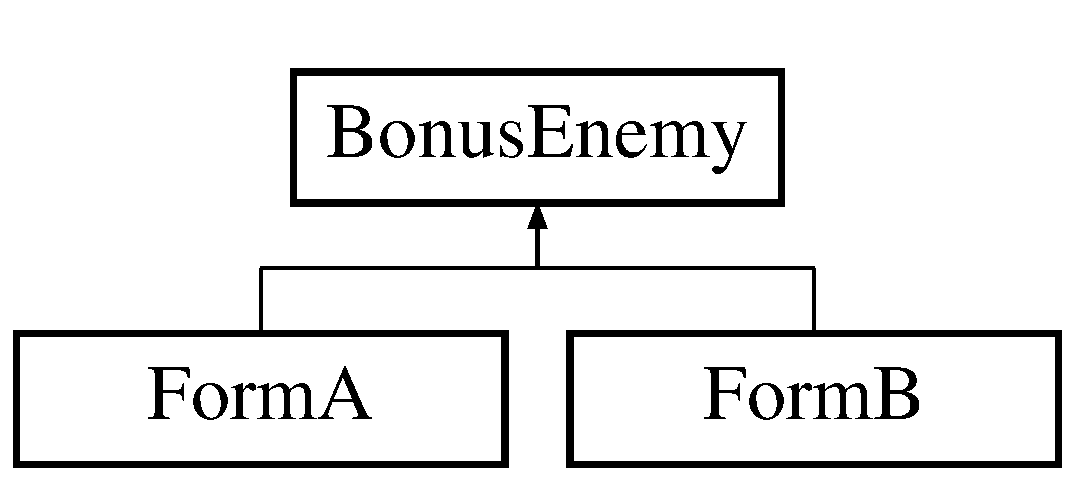
\includegraphics[height=2.000000cm]{class_bonus_enemy}
\end{center}
\end{figure}
\subsection*{Public Member Functions}
\begin{DoxyCompactItemize}
\item 
\hypertarget{class_bonus_enemy_ab49823c6432f006fe18018f1e39959e0}{void {\bfseries set\+Enemy\+Health} ()}\label{class_bonus_enemy_ab49823c6432f006fe18018f1e39959e0}

\item 
\hypertarget{class_bonus_enemy_a5bcfb846c3ee4c2254f7508473ec5659}{virtual void {\bfseries attack} ()}\label{class_bonus_enemy_a5bcfb846c3ee4c2254f7508473ec5659}

\item 
\hypertarget{class_bonus_enemy_a4b5f78ccb9e79885033ba60f893d1491}{int {\bfseries get\+Enemy\+Health} () const }\label{class_bonus_enemy_a4b5f78ccb9e79885033ba60f893d1491}

\end{DoxyCompactItemize}
\subsection*{Protected Attributes}
\begin{DoxyCompactItemize}
\item 
\hypertarget{class_bonus_enemy_ae09f90f7cdb5c71740d9d2da96c437ee}{int {\bfseries enemy\+Health}}\label{class_bonus_enemy_ae09f90f7cdb5c71740d9d2da96c437ee}

\end{DoxyCompactItemize}


The documentation for this class was generated from the following file\+:\begin{DoxyCompactItemize}
\item 
Bonus\+Boss.\+h\end{DoxyCompactItemize}

\hypertarget{class_bonus_player}{\section{Bonus\+Player Class Reference}
\label{class_bonus_player}\index{Bonus\+Player@{Bonus\+Player}}
}
\subsection*{Public Member Functions}
\begin{DoxyCompactItemize}
\item 
\hypertarget{class_bonus_player_a7243fc1584f32f05c4b39f896816e5e3}{void {\bfseries set\+Bonus\+Player\+H\+P} (int damage)}\label{class_bonus_player_a7243fc1584f32f05c4b39f896816e5e3}

\item 
\hypertarget{class_bonus_player_aa4dd3d06dac86aa80b899b15e1545736}{int {\bfseries get\+Bonus\+Player\+H\+P} () const }\label{class_bonus_player_aa4dd3d06dac86aa80b899b15e1545736}

\end{DoxyCompactItemize}


The documentation for this class was generated from the following file\+:\begin{DoxyCompactItemize}
\item 
Bonus\+Boss.\+h\end{DoxyCompactItemize}

\hypertarget{class_foreign_time}{\section{Foreign\+Time Class Reference}
\label{class_foreign_time}\index{Foreign\+Time@{Foreign\+Time}}
}
Inheritance diagram for Foreign\+Time\+:\begin{figure}[H]
\begin{center}
\leavevmode
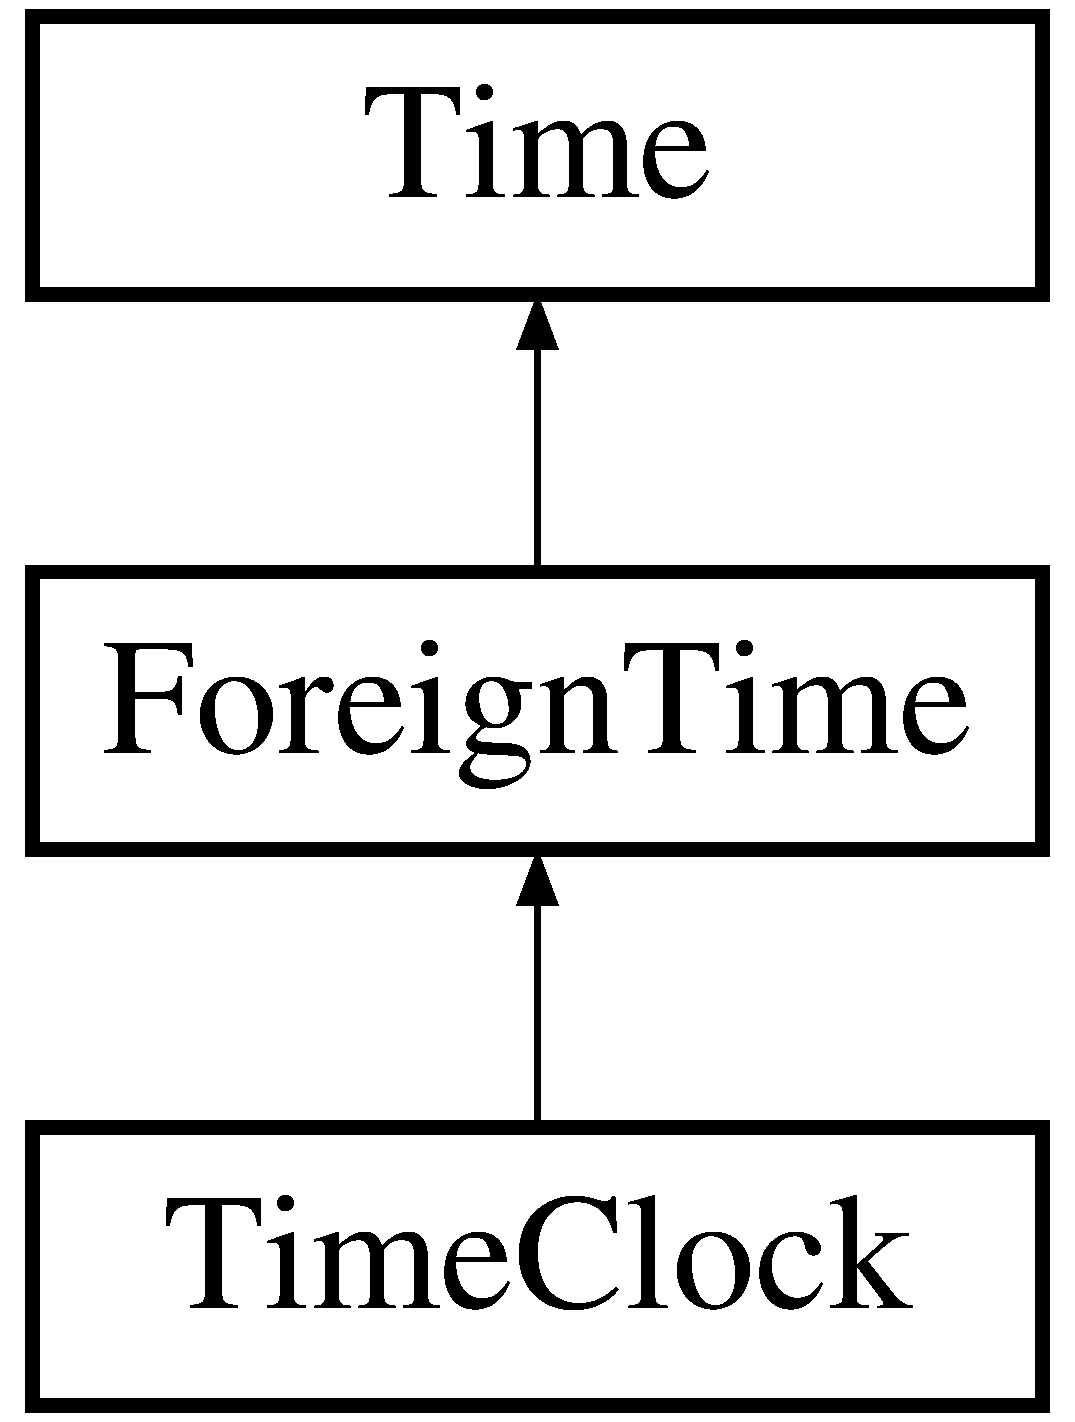
\includegraphics[height=3.000000cm]{class_foreign_time}
\end{center}
\end{figure}
\subsection*{Public Member Functions}
\begin{DoxyCompactItemize}
\item 
\hypertarget{class_foreign_time_a75e05233ce7712474f132818e441e89e}{{\bfseries Foreign\+Time} (int h, int s)}\label{class_foreign_time_a75e05233ce7712474f132818e441e89e}

\item 
\hypertarget{class_foreign_time_a2337883b85694c788de5a710d5721067}{void {\bfseries set\+Time} (int h, int s)}\label{class_foreign_time_a2337883b85694c788de5a710d5721067}

\item 
\hypertarget{class_foreign_time_a80bcae6da9b1367648f61ea4abd8dacd}{int {\bfseries Fore\+To\+Stand\+Hr} (int fore)}\label{class_foreign_time_a80bcae6da9b1367648f61ea4abd8dacd}

\item 
\hypertarget{class_foreign_time_a9d556acaadddd90891072922fba0ea7f}{int {\bfseries For\+To\+Stand\+Min} (int fore)}\label{class_foreign_time_a9d556acaadddd90891072922fba0ea7f}

\item 
\hypertarget{class_foreign_time_aaf4dd02db171d124570eabc8416ae8e2}{void {\bfseries get\+Hour} ()}\label{class_foreign_time_aaf4dd02db171d124570eabc8416ae8e2}

\item 
\hypertarget{class_foreign_time_a5e03d08c962435df282d97b317e12544}{void {\bfseries get\+Stand\+Hr} ()}\label{class_foreign_time_a5e03d08c962435df282d97b317e12544}

\end{DoxyCompactItemize}
\subsection*{Additional Inherited Members}


The documentation for this class was generated from the following file\+:\begin{DoxyCompactItemize}
\item 
Timing.\+h\end{DoxyCompactItemize}

\hypertarget{class_form_a}{\section{Form\+A Class Reference}
\label{class_form_a}\index{Form\+A@{Form\+A}}
}
Inheritance diagram for Form\+A\+:\begin{figure}[H]
\begin{center}
\leavevmode
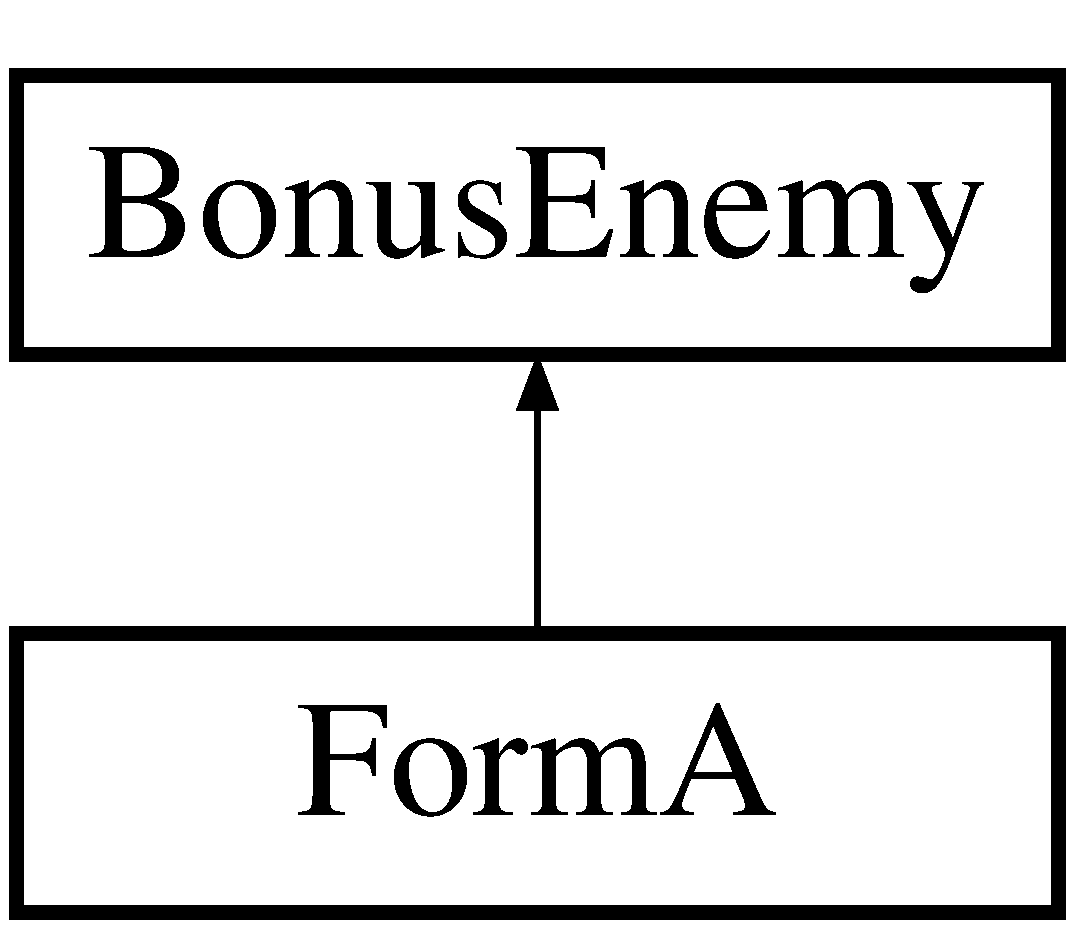
\includegraphics[height=2.000000cm]{class_form_a}
\end{center}
\end{figure}
\subsection*{Public Member Functions}
\begin{DoxyCompactItemize}
\item 
\hypertarget{class_form_a_aea7c6fc2a17ed6cf400878a2f53aeb96}{void {\bfseries attack} ()}\label{class_form_a_aea7c6fc2a17ed6cf400878a2f53aeb96}

\end{DoxyCompactItemize}
\subsection*{Additional Inherited Members}


The documentation for this class was generated from the following file\+:\begin{DoxyCompactItemize}
\item 
Bonus\+Boss.\+h\end{DoxyCompactItemize}

\hypertarget{class_form_b}{\section{Form\+B Class Reference}
\label{class_form_b}\index{Form\+B@{Form\+B}}
}
Inheritance diagram for Form\+B\+:\begin{figure}[H]
\begin{center}
\leavevmode
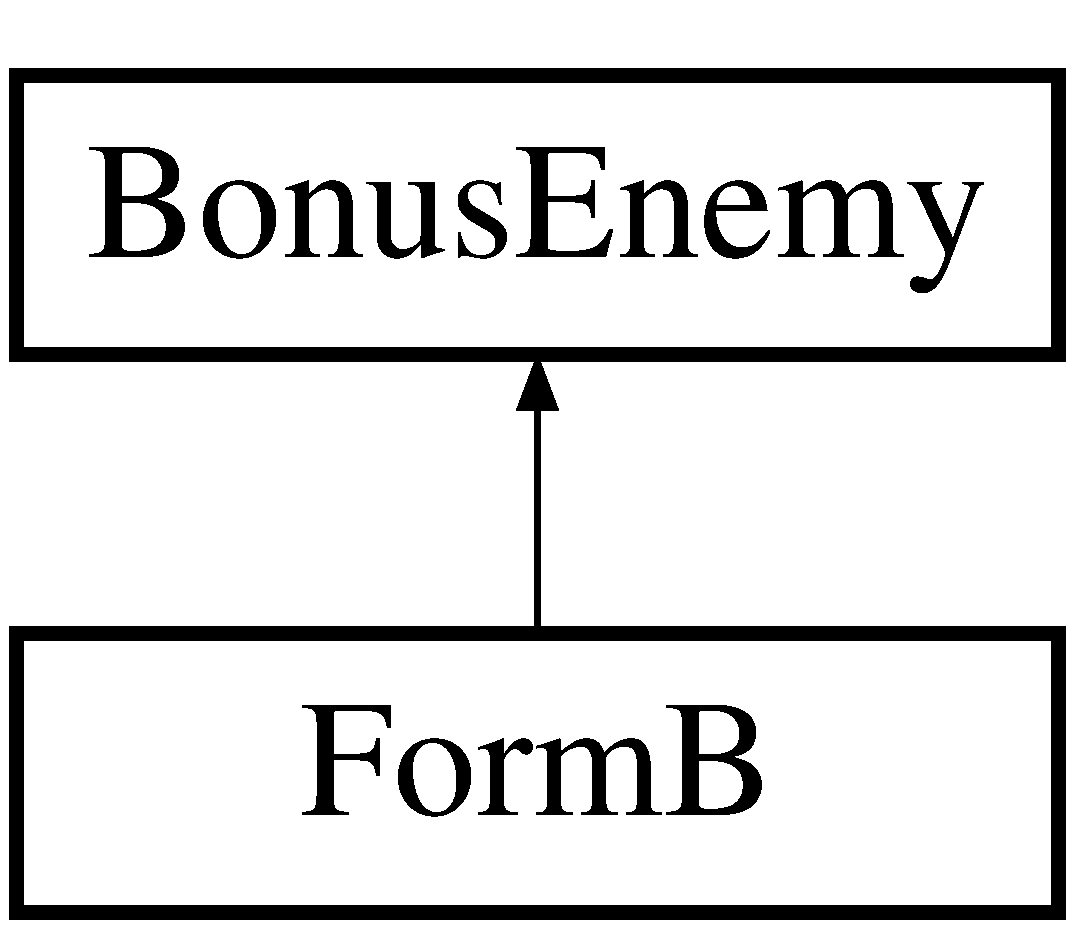
\includegraphics[height=2.000000cm]{class_form_b}
\end{center}
\end{figure}
\subsection*{Public Member Functions}
\begin{DoxyCompactItemize}
\item 
\hypertarget{class_form_b_a3d734a4f14d812c6336b718989350009}{void {\bfseries attack} ()}\label{class_form_b_a3d734a4f14d812c6336b718989350009}

\end{DoxyCompactItemize}
\subsection*{Additional Inherited Members}


The documentation for this class was generated from the following file\+:\begin{DoxyCompactItemize}
\item 
Bonus\+Boss.\+h\end{DoxyCompactItemize}

\hypertarget{struct_play}{\section{Play Struct Reference}
\label{struct_play}\index{Play@{Play}}
}
\subsection*{Public Attributes}
\begin{DoxyCompactItemize}
\item 
int $\ast$ \hyperlink{struct_play_ac937f89a2cff0d973be6a7996d327d69}{player\+Damage}
\item 
int \hyperlink{struct_play_acd4b4302358063ac72cb35f970096a5a}{player\+Health}
\item 
char \hyperlink{struct_play_a4d9060044c087e729eaf90363683a136}{user\+Name} \mbox{[}$\,$\mbox{]}
\end{DoxyCompactItemize}


\subsection{Member Data Documentation}
\hypertarget{struct_play_ac937f89a2cff0d973be6a7996d327d69}{\index{Play@{Play}!player\+Damage@{player\+Damage}}
\index{player\+Damage@{player\+Damage}!Play@{Play}}
\subsubsection[{player\+Damage}]{\setlength{\rightskip}{0pt plus 5cm}int$\ast$ Play\+::player\+Damage}}\label{struct_play_ac937f89a2cff0d973be6a7996d327d69}
\hypertarget{struct_play_acd4b4302358063ac72cb35f970096a5a}{\index{Play@{Play}!player\+Health@{player\+Health}}
\index{player\+Health@{player\+Health}!Play@{Play}}
\subsubsection[{player\+Health}]{\setlength{\rightskip}{0pt plus 5cm}int Play\+::player\+Health}}\label{struct_play_acd4b4302358063ac72cb35f970096a5a}
\hypertarget{struct_play_a4d9060044c087e729eaf90363683a136}{\index{Play@{Play}!user\+Name@{user\+Name}}
\index{user\+Name@{user\+Name}!Play@{Play}}
\subsubsection[{user\+Name}]{\setlength{\rightskip}{0pt plus 5cm}char Play\+::user\+Name\mbox{[}$\,$\mbox{]}}}\label{struct_play_a4d9060044c087e729eaf90363683a136}


The documentation for this struct was generated from the following file\+:\begin{DoxyCompactItemize}
\item 
C\+:/\+Users/\+Kevin Vo/\+Documents/\+Net\+Beans\+Projects/\+Vo\+\_\+\+Kevin\+\_\+\+Project\+\_\+1 \+\_\+48130/\hyperlink{main_8cpp}{main.\+cpp}\end{DoxyCompactItemize}

\hypertarget{class_sortable_vector}{\section{Sortable\+Vector$<$ T $>$ Class Template Reference}
\label{class_sortable_vector}\index{Sortable\+Vector$<$ T $>$@{Sortable\+Vector$<$ T $>$}}
}
\subsection*{Public Member Functions}
\begin{DoxyCompactItemize}
\item 
\hypertarget{class_sortable_vector_a368abcd55b20725f5432ed59ceaf32c9}{{\bfseries Sortable\+Vector} (int)}\label{class_sortable_vector_a368abcd55b20725f5432ed59ceaf32c9}

\item 
\hypertarget{class_sortable_vector_a4fc7e88ad62df25f52674c61b49ab402}{{\bfseries Sortable\+Vector} (const \hyperlink{class_sortable_vector}{Sortable\+Vector} \&)}\label{class_sortable_vector_a4fc7e88ad62df25f52674c61b49ab402}

\item 
\hypertarget{class_sortable_vector_a32c7457f2f4ad2c5a2d8a8fca159b54f}{int {\bfseries size} () const }\label{class_sortable_vector_a32c7457f2f4ad2c5a2d8a8fca159b54f}

\item 
\hypertarget{class_sortable_vector_a0d213de9ff82359a9ee30ddb5943970e}{T {\bfseries get\+Value} (int position)}\label{class_sortable_vector_a0d213de9ff82359a9ee30ddb5943970e}

\item 
\hypertarget{class_sortable_vector_a49e1016ea43758b84d02424faa9d8e61}{void {\bfseries sorter} ()}\label{class_sortable_vector_a49e1016ea43758b84d02424faa9d8e61}

\item 
\hypertarget{class_sortable_vector_a4bcb40b523a26311ce73719321e4818e}{T \& {\bfseries operator\mbox{[}$\,$\mbox{]}} (const int \&)}\label{class_sortable_vector_a4bcb40b523a26311ce73719321e4818e}

\end{DoxyCompactItemize}


The documentation for this class was generated from the following file\+:\begin{DoxyCompactItemize}
\item 
Sort.\+h\end{DoxyCompactItemize}

\hypertarget{class_time}{\section{Time Class Reference}
\label{class_time}\index{Time@{Time}}
}
Inheritance diagram for Time\+:\begin{figure}[H]
\begin{center}
\leavevmode
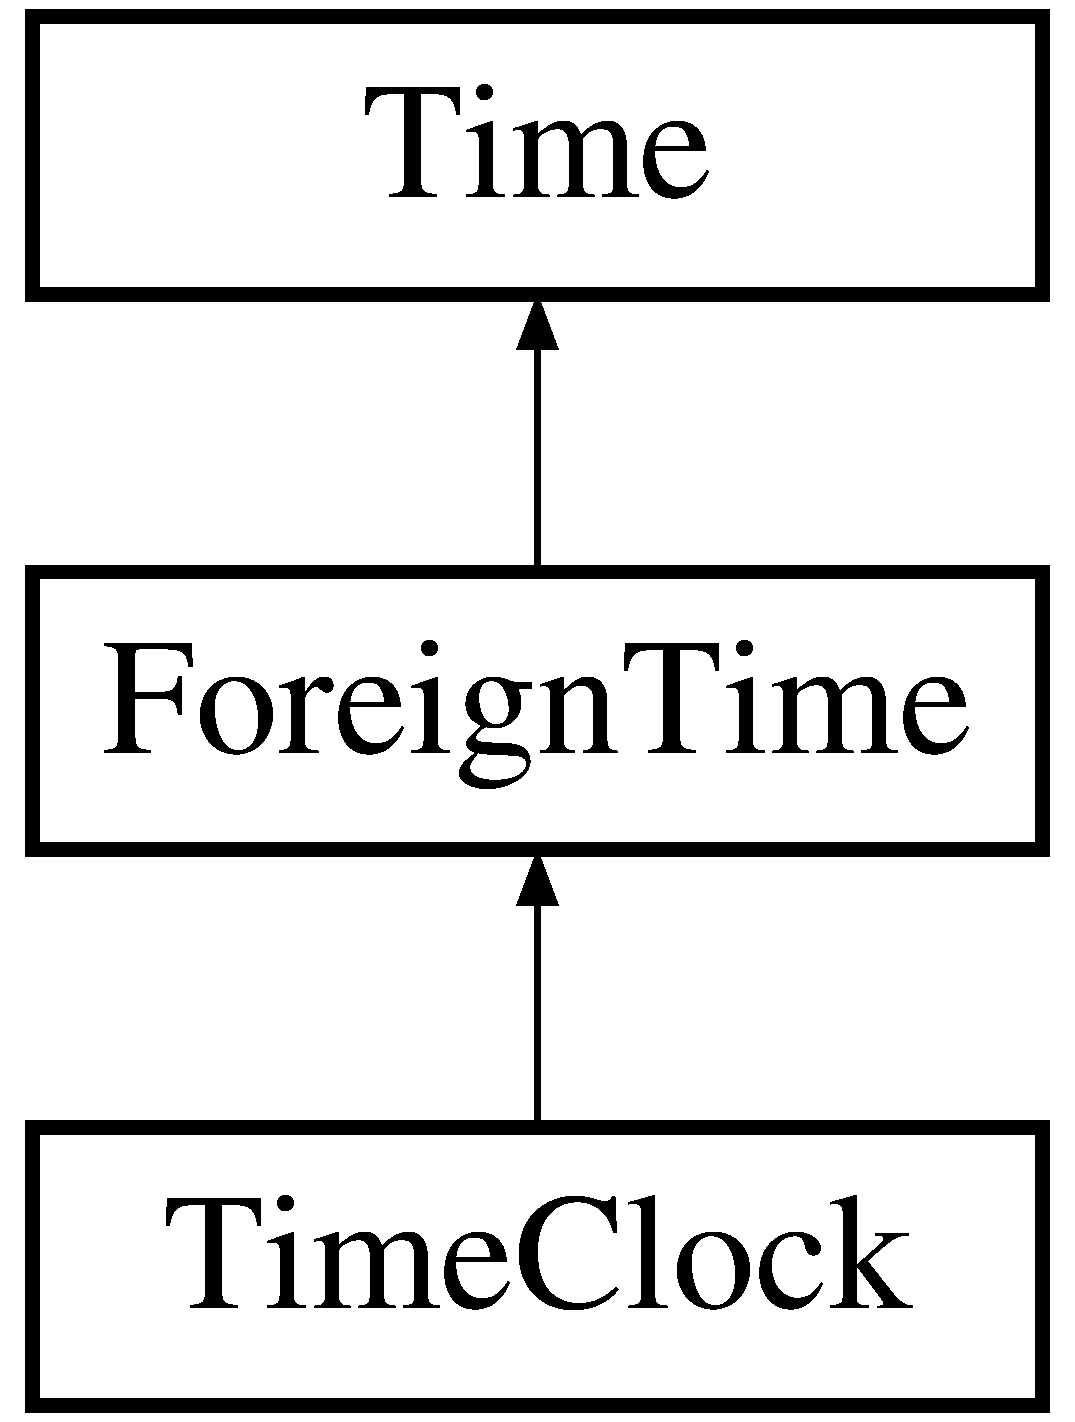
\includegraphics[height=3.000000cm]{class_time}
\end{center}
\end{figure}
\subsection*{Public Member Functions}
\begin{DoxyCompactItemize}
\item 
\hypertarget{class_time_a92491fd96ed1f4735d053080e3e47a32}{{\bfseries Time} (int h, int m, int s)}\label{class_time_a92491fd96ed1f4735d053080e3e47a32}

\item 
\hypertarget{class_time_ae05f94882a72debabb02e0889054d89a}{void {\bfseries set\+Time} (int h, int m, int s)}\label{class_time_ae05f94882a72debabb02e0889054d89a}

\item 
\hypertarget{class_time_ae0ce1e970c739d756282c95ebe458baf}{int {\bfseries get\+Hour} ()}\label{class_time_ae0ce1e970c739d756282c95ebe458baf}

\item 
\hypertarget{class_time_ac258de15a1a13d73c94ac06929899321}{int {\bfseries get\+Min} ()}\label{class_time_ac258de15a1a13d73c94ac06929899321}

\item 
\hypertarget{class_time_a07916f5becb53f92a29bcb02b11b7c3b}{int {\bfseries get\+Sec} ()}\label{class_time_a07916f5becb53f92a29bcb02b11b7c3b}

\end{DoxyCompactItemize}
\subsection*{Protected Attributes}
\begin{DoxyCompactItemize}
\item 
\hypertarget{class_time_a497d35aa44ea40706dbab08f7a31d069}{int {\bfseries hour}}\label{class_time_a497d35aa44ea40706dbab08f7a31d069}

\item 
\hypertarget{class_time_aa76ccbe1c5b4f22472247fd517b1a903}{int {\bfseries min}}\label{class_time_aa76ccbe1c5b4f22472247fd517b1a903}

\item 
\hypertarget{class_time_a348691e37ae949e13b2c19f8db461c0e}{int {\bfseries sec}}\label{class_time_a348691e37ae949e13b2c19f8db461c0e}

\end{DoxyCompactItemize}


The documentation for this class was generated from the following file\+:\begin{DoxyCompactItemize}
\item 
Timing.\+h\end{DoxyCompactItemize}

\hypertarget{class_time_clock}{\section{Time\+Clock Class Reference}
\label{class_time_clock}\index{Time\+Clock@{Time\+Clock}}
}
Inheritance diagram for Time\+Clock\+:\begin{figure}[H]
\begin{center}
\leavevmode
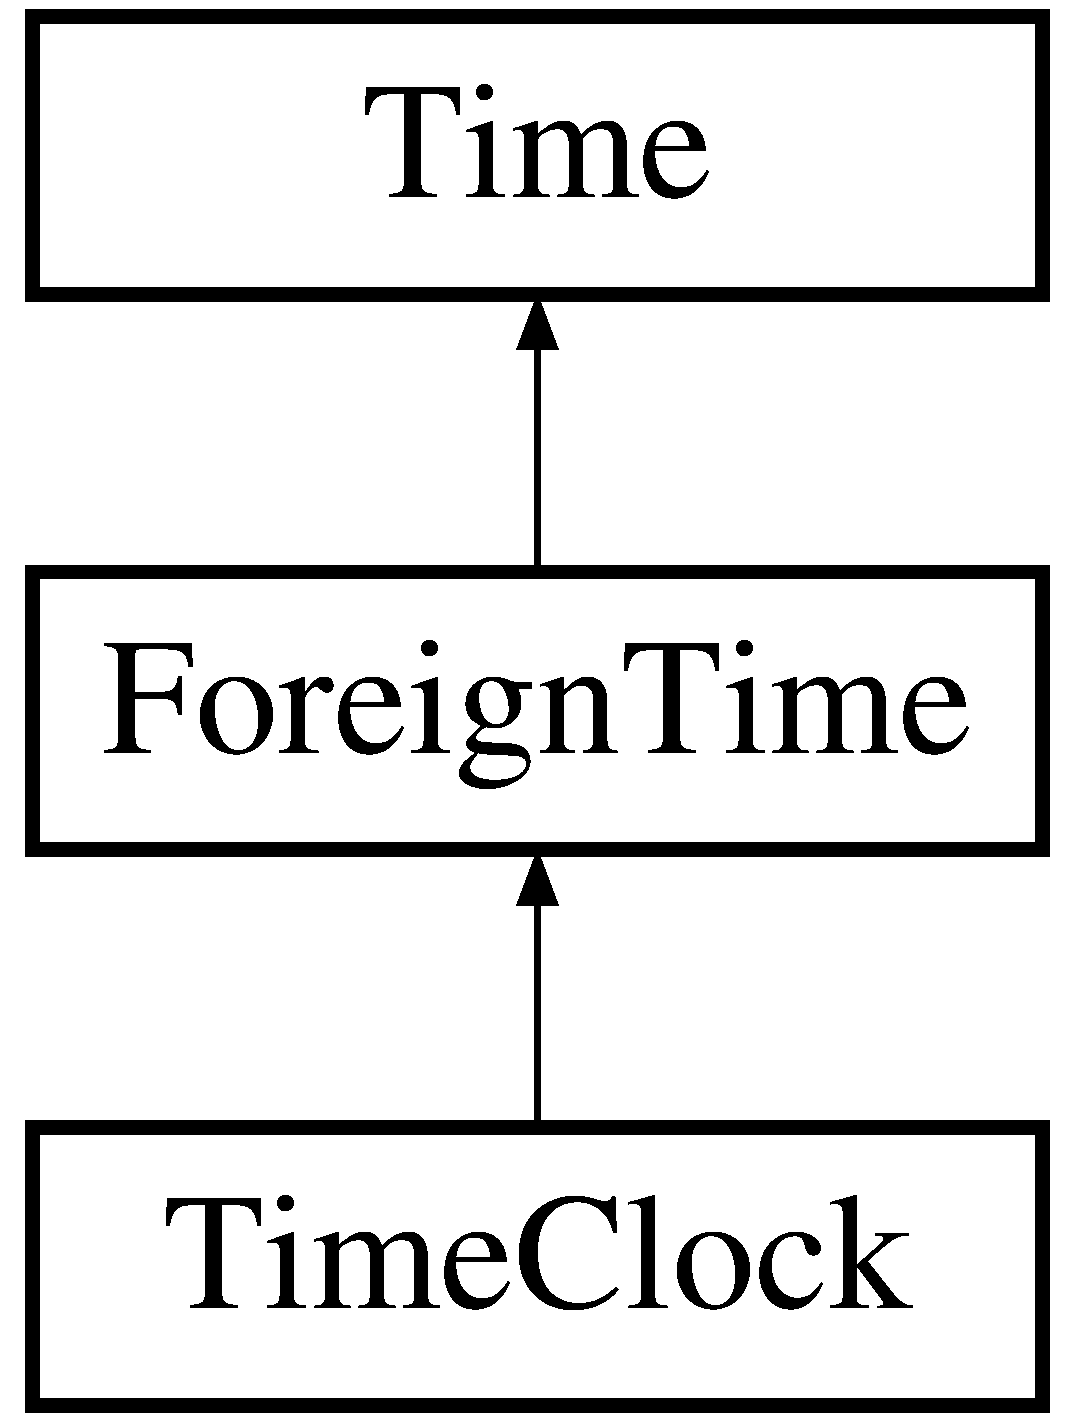
\includegraphics[height=3.000000cm]{class_time_clock}
\end{center}
\end{figure}
\subsection*{Public Member Functions}
\begin{DoxyCompactItemize}
\item 
\hypertarget{class_time_clock_ae6a3e28c5b3b5d38ee31deb6e197a67a}{{\bfseries Time\+Clock} (int time1, int time2)}\label{class_time_clock_ae6a3e28c5b3b5d38ee31deb6e197a67a}

\item 
\hypertarget{class_time_clock_acaa3cf5befe263aa89ceb8967862b560}{void {\bfseries display} ()}\label{class_time_clock_acaa3cf5befe263aa89ceb8967862b560}

\end{DoxyCompactItemize}
\subsection*{Additional Inherited Members}


The documentation for this class was generated from the following file\+:\begin{DoxyCompactItemize}
\item 
Timing.\+h\end{DoxyCompactItemize}

%--- End generated contents ---

% Index
\newpage
\phantomsection
\addcontentsline{toc}{chapter}{Index}
\printindex

\end{document}
